%
%
\documentclass[11pt]{scrartcl}

% own geometry
%\usepackage[a4paper, left=3cm, right=3cm]{geometry}

\usepackage[ngerman]{babel} 
\usepackage[utf8]{inputenc} 
\usepackage[T1]{fontenc}
\usepackage{graphicx}
\usepackage{color}
\usepackage{xcolor}
\usepackage{jurabib}
\usepackage{hyperref}

\renewcommand*{\jbauthorfont}{\textsc}
\renewcommand*{\bibfnfont}{\normalfont}
\renewcommand*{\biblnfont}{\textsc}
%\renewcommand*{\samepageibidemname}{Ebd.}
\renewcommand*{\bibbtsep}{In: }
\renewcommand*{\bibjtsep}{In: }
\renewcommand*{\bibpldelim}{(}
\renewcommand*{\biburlprefix}{}
\renewcommand*{\biburlsuffix}{}

\makeatletter
\renewcommand*{\jbshorttitlefont}{%
\ifthenelse{%
\equal{\jb@@type}{article}%
\or
\equal{\jb@@type}{periodical}%
\or
\equal{\jb@@type}{incollection}%
}{%
\upshape%
}{%
\textit%
}%
}
\makeatother

\renewcommand*{\bibprdelim}{)}
\renewcommand*{\ajtsep}{}
\renewcommand*{\bpubaddr} { :}
\renewcommand*{\jbbtasep} { ; }
\renewcommand*{\jbbfsasep} { ; }
\renewcommand*{\jbbstasep} { ; }
\renewcommand*{\bibbtasep} { ; }
\renewcommand*{\bibbfsasep} { ; }
\renewcommand*{\bibbstasep} { ; } %between second and third author sep
\renewcommand*{\jbbtesep} { ; } %between two editors sep
\renewcommand*{\jbbfsesep} { ; } %between first and second editor sep
\renewcommand*{\jbbstesep} { ; } %between second and third editor sep
\renewcommand*{\bibbtesep} { ; } %between two editors sep
\renewcommand*{\bibbfsesep} { ; } %between first and second editor sep
\renewcommand*{\bibbstesep} { ; } %between second and third editor sep
\AddTo\bibsgerman{\def\editorsname{(Hrsg.)}}
\AddTo\bibsgerman{\def\editorname{(Hrsg.)}}
%\jurabibsetup{super, citefull=first,ibidem}
%\jurabibsetup{ibidem}
%\jurabibsetup{authorformat=citationreversed}
%\jurabibsetup{authorformat=reducedifibidem}
\jurabibsetup{biblikecite}
%\jurabibsetup{bibformat=ibidem}
%\jurabibsetup{pages=always}
\jbfirstcitepageranges
\AddTo\bibsgerman{\def\herename{hier}}
\jbuseidemhrule

\jurabibsetup{
  authorformat={smallcaps,year,and,citationreversed},
  titleformat={colonsep,all,italic},
  commabeforerest,
  see,
  dotafter=bibentry,
  ibidem=strict,
  biblikecite
}

\renewcommand*{\bibbtasep}{ und } %
\renewcommand*{\bibbfsasep}{, }   %
\renewcommand*{\bibbstasep}{ und }
\renewcommand*{\jbtitlefont}{}
\renewcommand*{\bibtfont}{}
\renewcommand*{\bibbtfont}{}
\renewcommand*{\bibjtfont}{}
\renewcommand*{\bibapifont}{}
\renewcommand*{\jbshorttitlefont}{}



	%
	% CITATIONS
	%
\newcommand{\book}[2]{\footnote{\cite[Vgl.][#2]{#1}}}
\newcommand{\bookwf}[2]{\cite[Vgl.][#2]{#1}}
\newcommand{\bookdir}[2]{\footnote{\cite[][#2]{#1}}}
\newcommand{\inetwf}[1]{\cite[Vgl.][\citefield{url}{#1}]{#1}}
\newcommand{\inetwfdir}[1]{\cite[][\citefield{url}{#1}]{#1}}
\newcommand{\inet}[1]{\footnote{\inetwf{#1}}}
\newcommand{\inetdir}[1]{\footnote{\cite[][\citefield{url}{#1}]{#1}}}
\newcommand{\innerref}[1]{\footnote{Vgl. auch Kapitel \ref{#1} dieser Arbeit, S. \pageref{#1}}}
\newcommand{\vgl}[2]{\cite[Vgl.][#2]{#1}}
\newcommand{\citeauthoryear}[1]{\citeauthor{#1} (\citeyear{#1})}
\bibliographystyle{jurabib}

% setup of source code listings
\usepackage{listings}
%\usepackage{courier}
\usepackage{caption}
\lstset{
	basicstyle=\footnotesize\ttfamily,	% default font
	numbers=left,						% line numbers placement
	numberstyle=\tiny,					% line numbers style
	%stepnumber=2,						% line number padding
	numbersep=5pt,						% padding between line numbers and code
	tabsize=2,							% 
	extendedchars=true,         
	breaklines=true,						% line breaks 
	keywordstyle=\color{red},
	frame=b,
	stringstyle=\color{white}\ttfamily,	% color of strings in code
	showspaces=false,					% visualize spaces
    showtabs=false,						% visualize tabs
    xleftmargin=17pt,
	framexleftmargin=17pt,
	framexrightmargin=5pt,
	framexbottommargin=4pt,
	showstringspaces=false				% visualize spaces in strings        
 }
 
 \lstloadlanguages{% Check docs for further languages ...
         C,
         C++
 }

\setlength{\parindent}{0pt}
\setlength{\parskip}\medskipamount

\DeclareCaptionFont{white}{\color{white}}
\DeclareCaptionFormat{listing}{\colorbox{gray}{\parbox{\textwidth}{#1#2#3}}}
\captionsetup[lstlisting]{format=listing,labelfont=white,textfont=white}

% layout the box
%\DeclareCaptionFormat{listing}{\colorbox[rgb]{0.43, 0.35, 0.35 {\parbox{\textwidth}{\hspace{15pt}#1#2#3}}}

% layout the caption ontop of code
\captionsetup[lstlisting]{format=listing,labelfont=white,textfont=white, singlelinecheck=false, margin=0pt, font={bf,footnotesize}}

% Headings
\usepackage{fancyhdr}
\fancyhead[R]{\colorbox{blue!20}{ Oliver Erxleben}}
\fancyfoot{}

% Document begins now
\begin{document}

\author{%
	Martin Helmich \small(\href{mailto:martin.helmich@hs-osnabrueck.de}{martin.helmich@hs-osnabrueck.de})\\%
	Oliver Erxleben \small(\href{mailto:oliver.erxleben@hs-osnabrueck.de}{oliver.erxleben@hs-osnabrueck.de})\\ \\%
	%
	Hochschule Osnabr"uck \\%
	Ingenieurswissenschaften und Informatik \\%
	Informatik - Mobile und Verteilte Anwendungen }

\title{
\includegraphics[scale=0.75,keepaspectratio]{img/hs_os.png}\linebreak \linebreak Parallelisierung mit OpenMP}

\maketitle
\thispagestyle{empty}
\tableofcontents

\begin{abstract}

\end{abstract}


\pagebreak
% set new page style
\pagestyle{fancy}
% hoooray page 1! begins 
\setcounter{page}{1} 

\section{OpenMP} Open Multi-Processing (kurz: OpenMP) ist eine Programmierschnittstelle
f"ur die Sprachen C/C++ und Fortran, welche seit 1997 von unterschiedlichen Hardware- und Compilerherstellern
entwickelt wird. Ziel von OpenMP, welches mittlerweile den Versionsstand 3.1 erreicht hat, ist es ein portables und zugleich paralleles
Programmiermodell f"ur Shared-Memory-Architekturen\footnote{Shared-Memory-Architektur: } zur Verf"ugung zu stellen. Es setzt sich aus Compilerdirektiven, Bibliotheksfunktionen und Umgebungsvariablen zusammen. Anders als viele alternative Ansätze zur Parallelisierung von Programmen sind nur wenige Änderungen an sequenziellen Programmen notwendig um parallele Abläufe zu implementieren. Auch die Lesbarkeit des parallelisierten Quelltextes wird im Vergleich zu anderen alternativen Ansätzen stark verbessert.\footnote{Vgl. \cite{openmp08} }

Ein weiteres Plus f"ur den Einsatz von OpenMP ist die weite Verbreitung von Multi-Core-Rechnern und die Implementierung in vielen verbreiteten Compilern. So ist OpenMP im GCC seit der Version 4.2, im Visual Studio C/C++ Compiler seit der Version 2005 oder im Intel C/C++-Compiler seit Version 8 verf"ugbar. Compiler die keine OpenMP-Unterst"utzung bieten, ignorieren aufgrund der Pragma-Compilerdirektiven die Ausf"uhrung als parallelisierte OpenMP-Implementierung, was zu einer guten Portabilität f"uhrt.

Ursprünglich wurde OpenMP für den Bereich High Performance Computing entwickelt, wo Programmcode meist viele Schleifen enthält. Demnach ist die Parallelisierung von Schleifen die Hauptaufgabe von OpenMP und die meisten Vorteile können an dieser Stelle von OpenMP aufgezeigt werden. 
% TODO: Beispiel einfügen??

\subsection{Merkmale von OpenMP}

Mit OpenMP wird ein hoher \textbf{Abstraktionsgrad} erreicht, da Threads nicht durch einen Programmierer initialisiert, gestartet oder beenden werden m"ussen. Wie bereits in der Einf"uhrung erwähnt, beitet OpenMP eine gute \textbf{Portabilität} des Programms an, zum einen ist OpenMP in vielen Mainstream-Compilern implementiert, zum anderen können Compiler ohne OpenMP-Unterst"utzung das Programm ohne Veränderung kompilieren, da die Compilerdirektiven durch Pragmas eingesetzt und ignoriert werden können. Auch bleibt der sequenzielle Programmcode vollständig erhalten, wenn nicht mittels OpenMP kompiliert wird. Der Quelltext kann somit \textbf{Schrittweise parallelisiert} werden. 

\subsection{Ausführungsmodell}

Die parallele Ausf"uhrung erfolgt durch Threads auf dem
Fork-/Join\footnote{Fork/Join:}-Ausf"uhrungsmodell. Zu Beginn eines Programms ist nur ein Thread aktiv, der sog. \textit{Master Thread}. Sobald bei der Programmausf"uhrung die Direktive \textit{\#pragma omp parallel \{ ... \} } erreicht wird, gabelt sich die
Ausf"uhrung in Threads auf. Die erstellten Threads werden als \textit{Threadteam} oder \textit{team of threads}
bezeichnet\footnote{Die Implementierung von OpenMP entscheidet "uber die Art der Threads die erstellt werden. Es könnten Threds auf Basis der PThreads-Bibliothek oder aber auch als vollwertige Shared-Memory-Prozesse umgesetzt sein.}. F"ur OpenMP, bzw. der Entwicklung mit OpenMP stellen Threads einen Kontrollfluss mit gemeinsamen Adressraum dar.

Die schließende geschweifte Klammer ist zudem ein Synchronisationspunkt, andem das team of threads auf alle Teammitglieder wartet. Die Abbildung \ref{join_fork_model} stellt einen möglichen Ablauf mit OpenMP dar.

Sofern nicht anders angegeben verwenden alle Threads eines Thread-Teams einen gemeinsam genutzten Adressraum und können somit auf alle Variablen eines parallen Codeabschnitts zugreifen, über die auch die Kommunikation zwischen den Threads ermöglicht wird. Folgende Klauseln für Variablen können eingesetzt werden:

\begin{itemize}
\item \textit{shared}/\textit{private}: Threads können explizit als gemeinsame Variable oder für jeden Thread private Variable deklariert werden.
\item \textit{firstprivate}/\textit{lastprivate}: Diese Klauseln erlauben die Initialisierung, bzw. Finalisierung der Variable beim Ein- und Austritt in oder aus einem parallen Bereich.
\item \textit{default}: Das Standardverhalten kann verändert werden. % TODO nochmal prüfen
\item \textit{reduction}: Eine spezielle gemeinsam genutzte Variable über die mehrere Threads Wrte zusammentragen können.
\end{itemize}


\begin{figure}[h!]
\centering
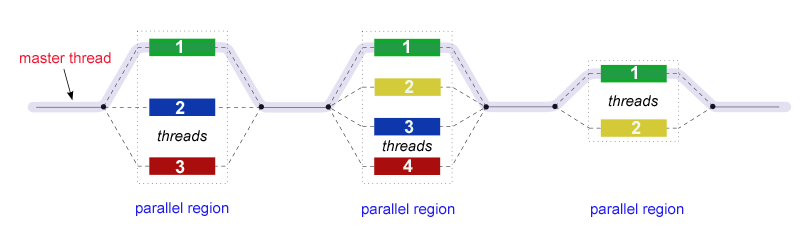
\includegraphics[width=1.0\textwidth]{img/fork_join.png}
\label{join_fork_model}
\caption{Fork-Join-Prinzip}
\protect{\textit{Entnommen aus OpenMP Tutorial} (siehe \cite{openmptut12})}
\end{figure} 

\subsection{Umgebungsvariablen und Bibliotheksfunktionen}




\subsection{Parallelisierung von Schleifen} 
Nach der Klassifikation von Flynn kann OpenMP als Single Programm Multiple Data (SPMD) beschrieben werden. Demnach führt jeder Thread der gestartet wurde den Schleifenblock aus. Dabei hat jeder Thread seine eigene Iteration und Teilmenge von Daten.\textit{(Vgl. siehe \cite{openmp08}, Kapitel 3.1: Parallelität auf Schleifenebene)}

Ein team of threads wird mittels \textit{\#pragma omp parallel} gestartet. Zur Veranschaulichung sei das Listing \ref{parallelExample} gegeben. 

\lstinputlisting[caption= pragma omp parallel - Beispiel, label=parallelExample]{../src/1_3_example/parallel.c}
Die For-Schleife in Zeile 8 wird von allen vom System zur Verfügung stehenden Threads ausgeführt. Allerdings teilen sich die Threads nicht die Arbeit, sondern jeder Thread führt die Schleife komplett für sich aus. Um eine Schleife parallel auszuführen, muss über eine weitere Direktive, wie in Listing \ref{parallelForExample} zu sehen, eingefügt werden. 

\lstinputlisting[caption= pragma omp parallel for - Beispiel, label=parallelForExample]{../src/1_3_example/parallelfor.c}
In diesem Beispiel wird der zu parallelisierende Bereich eine Variable \textit{tid}, die threadId, übergeben. Jeder Thread erhält diese Variable, die nicht gemeinsam genutzt werden kann (private). Mittels \textit{\#pragma omp for} wird dem Compiler mitgeteilt das die darauffolgende Schleife parallel durch das team of threads  im parallelen Bereich ausgeführt werden soll.

Als Vorraussetzung für parallelisierbare Schleifen fordert OpenMP, dass Schleifen in kanonischer Form geschrieben sein müssen. Die kanonische Form liegt wenn folgende Bedingungen erfüllt sind: 
\begin{itemize}
\item Anzahl der Schleifendurchläufe muss berechnbar sein und darf sich innerhalb des Schleifenblocks nicht ändern. Ebenso dürfen sich Start und Endwert während des Schleifendurchlaufs nicht ändern.
\item Es sind nur boolsche Vergleichoperator im Schleifenkopf erlaubt.
\item Das Inkrement im Schleifenkopf darf nur aus Addition oder Subtraktion inkrementiert oder dekrementiert werden. 
\item \textbf{break}-Anweisungen dürfen nicht im Schleifenrumpf verwendet werden. Allerdings kann eine Iteration durch eine \textbf{continue}-Anweisung übergangen werden oder das gesamte Programm mittel \textbf{exit} verlassen werden.
\end{itemize}

Ein team of threads durch ihren gemeinsamen Adressraum synchronisiert. Dabei ist die Reihenfolge der Bearbeitung der Arbeit nicht "vorhersehbar". Um einen kritischen Adressraum innerhalb eines parallelen Abschnitts zu kennzeichnen, bietet OpenMP ein weitere Direktive an: \textit{\#pragma omp critical \{ ... \}}. Der von der Klammer umschlossene Code wird demnach von nur einem Thread ausgeführt. 

\subsection{Sections und Tasks}

Neben der Parallelisierung von Schleifen stellt sich auch die Frage der Arbeitsverteilung mittels OpenMP. 

\textbf{Sections} sind eine Möglichkeit Aufgaben innerhalb eines Threadteams ohne Schleifen zu verteilten. 

Das \textbf{Tasks}-Konzept ist die Hauptaktualisierung für OpenMP mit de Release der Version 3.0 gewesen. 


% TODO: Code Examples 

\pagebreak % first part ends

%\section{Vergleich mit TBB und anderen?!}

%\pagebreak % second part ends

\section{Untersuchung des Laufzeitverhaltens von OpenMP im Vergleich zur Intel TBB}
% renew to mark part of other team member
\fancyhead[R]{\colorbox{green!20}{ Martin Helmich}}

\subsection{Zielsetzung und Vorgehen}

Zielsetzung dieses Abschnittes ist es, die Möglichkeiten zur Parallelisierung eines sequentiellen Programms mit OpenMP
sowie die Leistungsfähigkeit und Skalierbarkeit von OpenMP im Vergleich zu Parallelisierungslösungen anderer Hersteller
zu untersuchen.

Als Beispiel dient dazu unser Beitrag zum von Intel ausgerichteten \emph{Accelerate Your Code}-Programmierwettbewerb vom
November 2012. Der Wettbewerbsbeitrag verwendet die Intel \emph{Threading Building Blocks}-Bibliothek (kurz TBB). Für
diese Arbeit wurde der Beitrag nach OpenMP portiert und anschließend das Laufzeitverhalten beider Programme untersucht
und verglichen.

Für die Messung der Laufzeit wurde das Programm \emph{GNU time} genutzt. Dieses misst die Zeit vom Starten bis zum Beenden eines Prozesses.\footnote{Vgl. \cite{time_man_2012}.}
Zur Messung des Speicherplatzverbrauchs wurde das Programm \emph{Massif} (ein Bestandteil des \emph{Valgrind}-Paketes) genutzt. Gemessen wurde jeweils der maximal an einem Zeitpunkt allozierte Speicher (Stack und Heap).\footnote{Vgl. \cite[S. 136ff.]{valgrind_2012}.}

Die Aufgabenstellung des Programmierwettbewerbs liegt in Anhang \ref{intel_ayc_problem} bei. Die Quelltexte beider
Programme liegen dieser Arbeit auf Datenträger bei.

\subsection{Auftretende Probleme}

Bei der Portierung des Programms von TBB auf OpenMP fiel vor allem der geringere Sprachumfang der OpenMP-Erweiterung
negativ auf.

Beispielsweise bietet die TBB eine (wenn auch nicht sonderlich effiziente)\footnote{Vgl. hierzu \cite{intel_cook_2012}:
Laut Handbuch stellt sich ein Parallelisierungsnutzen erst ab mehreren tausend Instruktionen pro Schleifendurchlauf
ein.} parallele While-Schleife in Form der \texttt{tbb::parallel\_do}-Methode. Ein vergleichbares OpenMP-Konstrukt
existiert nicht. Das Problem konnte gelöst werden, indem der iterative, mit einem Stack arbeitende, Algorithmus zurück
in eine rekursive Form überführt wurde. Diese konnte anschließend durch Task-Parallelität ohne Probleme parallelisiert
werden (Task-Parallelität wird sowohl von der TBB als auch von OpenMP unterstützt).

Ein weiteres Problem fiel bei der Implementierung des task-parallelen Algorithmus auf: Task-Parallelität wurde erst in
der Version 3.0 des OpenMP-Standards eingeführt.\footnote{Vgl. \cite[S.~134]{openmp08} und
\cite[S.~406ff]{ayguade_design_2009}.} Obwohl diese Version bereits 2008 veröffentlicht wurde,\footnote{Vgl.
\cite{openmp.org_openmp_2012}.} wird sie noch nicht von allen Compilern unterstützt. So verwendet MacOS X
beispielsweise auch 2012 noch die GCC-Version 4.2 von 2007 als Standard-Compiler. \emph{Visual C++} von Microsoft
unterstützt sogar in der aktuellen Version nur die Version 2.0 [!] des Standards.\footnote{Vgl.
\cite{openmp.org_openmp_2012-2} und
\cite{microsoft_openmp_2012}.}

Darüber hinaus fiel auf, dass die TBB zahlreiche hochentwickelte threadsichere Datenstrukturen anbietet (insbesondere
von der \texttt{tbb::concurrent\_hash\_map} wurde in der eingereichten Lösung des Intel-Wettbewerbs intensiver Gebrauch
gemacht). OpenMP hingegen bietet selbst keine entsprechenden Datenstrukturen an. Da die TBB jedoch explizit einen
Parallelbetrieb mit OpenMP gestattet,\footnote{Vgl. \cite{intel_mixing_2012}.} konnte das Problem gelöst werden, indem
auch in der OpenMP-Version des Programms die threadsicheren Datenstrukturen der TBB weiterverwendet wurden.

\subsection{Ergebnisse}

\subsubsection{Laufzeit}

Um die Leistungsfähigkeit der TBB- und OpenMP-Programme zu testen, wurde eine Eingabedatei mit 5 Millionen Flügen verwendet. Diese Eingabedatei wurde nicht von den Veranstaltern des Wettbewerbs zur Verfügung gestellt, sondern wurde im offiziellen Forum des Wettbewerbs von einem Teilnehmer angeboten. Die Verwendung einer Eingabedatei dieser Größe war jedoch notwendig, um überhaupt Unterschiede im Laufzeitverhalten beider Lösungen messen zu können.

Gemessen wurden Laufzeitverhalten und CPU-Auslastung des Programms in Abhängigkeit der zur Verfügung stehenden Threads (beginnend bei einem Thread bis hin zu 24 Threads). Das Laufzeitverhalten ist in Abbildung \ref{s13_runtime} auf Seite \pageref{s13_runtime} grafisch aufgetragen (jeder Datenpunkt ist das arithmetische Mittel aus je zehn Einzelmessungen). Die Laufzeit des TBB-Programms konvergiert hier gegen 21,33 Sekunden, die des OMP-Programms gegen 19,56 Sekunden.

Abbildung \ref{s13_speedup} auf Seite \pageref{s13_speedup} zeigt außerdem die Beschleunigung oder engl. \emph{Speed-Up}. Dieser ist nach \citeauthoryear{rauber_parallel_2010} wie folgt definiert:\footnote{Vgl. \cite[S.~162]{rauber_parallel_2010}.}

\begin{equation}
S_p(n) = \frac{T_1(n)}{T_p(n)}
\end{equation}

Der Speed-Up $S_p(5\cdot 10^6)$ des TBB-Programms konvergiert ab $p=12$ gegen einen Faktor von 3,91 und der des OMP-Programms gegen 4,29.

Die Effizienz beider Programme ist zudem in Abbildung \ref{s13_efficiency} auf Seite \pageref{s13_efficiency} gezeigt. Sie ist definiert wie folgt:\footnote{Vgl. \cite[S.~164]{rauber_parallel_2010}.}

\begin{equation}
E_p(n) = \frac{S_p(n)}{p} = \frac{T_1(n)}{p \cdot T_p(n)}
\end{equation}

\begin{figure}[pbt]
\centering
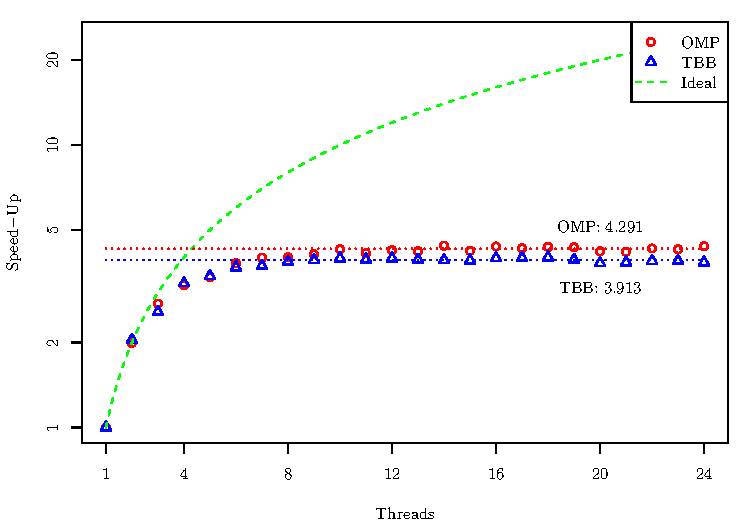
\includegraphics{../messdaten/s13_speedup.pdf}
\caption{Parallelisierungsgewinn $S_p(n)$, bei $n=5\cdot 10^6$ und $p \in [1;24]$.}
\label{s13_speedup}
\end{figure}

In der Auswertung fällt auf, dass die Laufzeit (und der davon abhängige Speed-Up) zügig konvergieren. Einerseits ist dies zweifellos darauf zurück zu führen, dass das Testsystem über 12 physikalische Rechenkerne verfügt; bei mehr als 12 Threads kann daher nur wenig zusätzlicher Nutzen durch weitere Threads erwartet werden. Andererseits fällt auf, dass die gemessene Laufzeit auch bei weniger als 12 Threads deutlich unter der idealen Laufzeit (hier angenommen als $T_{I,p}(n) = \frac{T_1(n)}{p}$) liegt.

Der geringere Speed-Up ist vermutlich auf sequentielle Anteile des Programms sowie erhöhten Synchronisationsbedarf durch Zugriff auf gemeinsame Datenstrukturen zurück zu führen. Diese Einflussfaktoren begrenzen nach dem \emph{Amdahlschen Gesetz} den maximal erreichbaren Speed-Up.\footnote{Vgl. \cite[S.~318]{bengel_masterkurs_2008}}

%Der geringere Speed-Up kann mit dem \emph{Amdahlschen Gesetz} erklärt werden. Dieses definiert den maximalen Speed-Up
%eines Programms wie folgt:\footnote{Vgl. \cite[S.~318]{bengel_masterkurs_2008}}

%\begin{equation}
%S_p(n) = \frac{T^*(n)}{f \cdot T^*(n) + \frac{1-f}{p}T^*(n)} = \frac{1}{f + \frac{1-f}{p}}
%\end{equation}

\subsubsection{Speicherverbrauch}

Zusätzlich zum Laufzeitverhalten wurde außerdem der Speicherverbrauch beider Implementierungen gemessen. Eine grafische Auswertung der Messergebnisse findet sich in Abbildung \ref{s14_memory} auf Seite \pageref{s14_memory}.

Es ist erkennbar, dass sich der Speicherverbrauch in Abhängigkeit zur Parallelisierung konstant verhält. In den durchgeführten Messungen lag der Speicherverbrauch der OMP-Implementierung mit im Mittel 174,615 MiB minimal höher als der der TBB-Implementier\-ung mit im Mittel 173,937 MiB.

\section{Fazit}

OpenMP stellt eine interessante Alternative zur bereits aus der Veranstaltung bekannten TBB-Bibliothek dar. Die Compiler-Direktiven von OpenMP sind nach eigener Auffassung einfacher handhabbar als die auf \emph{Function Objects} basierende TBB. Dies macht sich vor allem bei der Parallelisierung bereits bestehender, sequentieller Programme bemerkbar.

Negativ fällt im Vergleich zur TBB der etwas geringere Sprachumfang auf: So kennt OpenMP keine parallelen While-Schleifen und die Task-Parallelität, die insbesondere für die Parallelisierung irregulärer Probleme nötig ist,\footnote{Vgl. \cite[S.~6]{duran_tasking_2009}} wurde erst spät in den Standard aufgenommen und wird noch nicht von allen Compilern unterstützt.

Einen Vorteil OpenMPs gegenüber der TBB stellt der -- zwar geringe, aber dennoch messbare -- Geschwindigkeitsvorteil dar. In den durchgeführten Messungen konnte mit OpenMP bei hoher Parallelität ein um $\frac{4,291}{3,913}-1 = 9,66\%$ höherer Speed-Up erreicht werden. Hinsichtlich des Speicherverbrauchs sind keine relevanten Unterschiede messbar (der Speicherverbrauch von OpenMP war in der durchgeführten Messung um $1-\frac{173,937}{174,615} = 0,39\%$ höher, was praktisch jedoch vernachlässigbar ist).

Zusammenfassend eignet sich OpenMP ausgezeichnet zur Parallelisierung bereits besteh\-enden Codes. Die Compiler-Direktiven sind vergleichweise einfach handhabbar und erhalten die Lesbarkeit des ursprünglichen Quelltextes. Im Unteschied zur TBB beschränkt sich OpenMP zudem nicht auf C++, sondern ermöglicht auch die Parallelisierung von C-oder Fortran-Code.

Da OpenMP jedoch keine geeigneten threadsicheren Datenstrukturen mit sich bringt, empfiehlt sich die Verwendung von OpenMP zusammen mit einer entsprechenden Bibliothek (in C++ beispielsweise die TBB- oder die Boost-Bibliothek).

\pagebreak % third part ends

\fancyhead[R]{}

\thispagestyle{empty}
\listoffigures

\listoftables

\lstlistoflistings

\renewcommand*{\biburlprefix}{(URL: }
\renewcommand*{\biburlsuffix}{)}

\pagebreak
\addcontentsline{toc}{section}{Literaturverzeichnis} % Eintrag ins Inhaltsverzeichnis
\bibliography{bib/bib}

\appendix

\section{Aufgabenstellung des Intel Accelerate Your Code-Programmierwettbewerbs}

\label{intel_ayc_problem}

Es folgt ein Auszug aus:
\url{http://www.intel-software-academic-program.com/contests/ayc/2012-11/problem/Intel_AccelerateYourCode_2012-11_problem.pdf}

\begin{quote}
Let’s imagine you have to go to a software conference in San Francisco (lucky you !), you live in Berlin. Booking the cheapest flight is easy when you want to go from point A to point B and you know the dates. Several websites do that already.

But if you want to pay a little more to extend your flight and do some tourism, it’s getting complicated : you are interested in a lot of places (airports in Brazil, Mexico, Colombia, ...), and you are pretty flexible about the dates (before of after your conference). You just want to find a good opportunity : If I can get Berlin-San Francisco-SaoPaulo-Berlin for only 100 euros more than just Berlin-San Francisco-Berlin, I’ll spend a week there on vacation!

But most flights requires a layover (a stop), you have to deal with multiple airline companies, and the price of a single flight is varying depending on the company used for the other flights. If you take all the segments of a flights from a single company, it’s 30\% cheaper. Plus, companies are forming “alliances” to offer cheaper flights to the customers booking only inside the alliance. If you take all the segments of a flight from a single alliance, it’s 20\% cheaper.

Even today, this task requires human knowledge and skills because reservation software can’t handle the huge combinations. It could be automated. Customers would have more options, spend less time searching on websites, airlines would fill empty planes.

For this contest, you are given a first input file listing all the flights, and a second input file listing the alliances of companies (a company can be in several alliances).

A source file solving the problem, input files and expected outputs are given to help you start:\\
\url{http://www.intel-software-academic-program.com/contests/ayc/2012-11/problem/}

The goal is to optimize and parallelize the software. You can start from scratch if you want, but it’s probably safer to optimize and parallelize this reference version.

The goal is to optimize and parallelize for a wide range of use cases (few/many flights, few/many alliances, short/wide date ranges, ...).
\end{quote}

\section{Messung von Lautzeit und Speicherverbrauch}

\subsection{Grafische Auswertung der Messergebnisse}

\begin{figure}[pbt]
\centering
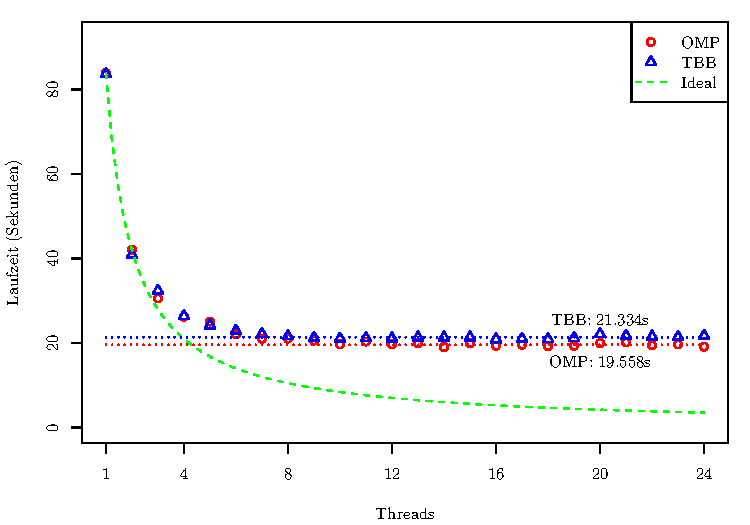
\includegraphics{../messdaten/s13_runtime.pdf}
\caption{Laufzeitverhalten $T_p(n)$, bei $n=5\cdot 10^6$ und $p \in [1;24]$.}
\label{s13_runtime}
\end{figure}

\begin{figure}[pbt]
\centering
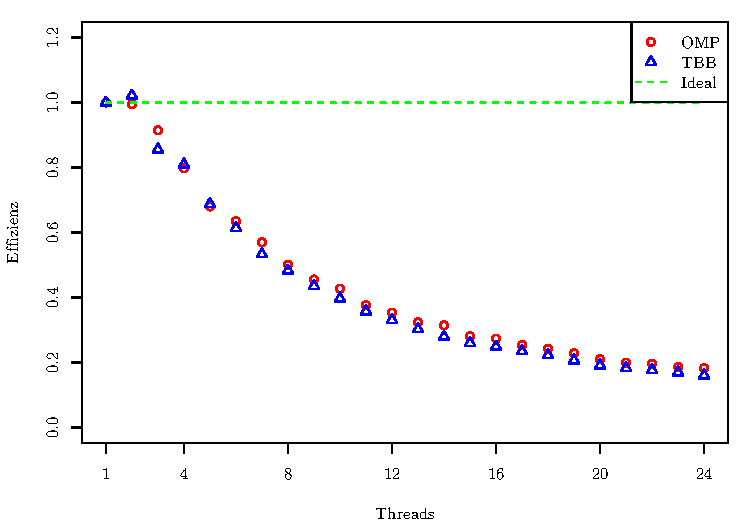
\includegraphics{../messdaten/s13_efficiency.pdf}
\caption{Effizienz $E_p(n)$, bei $n=5\cdot 10^6$ und $p \in [1;24]$.}
\label{s13_efficiency}
\end{figure}

\begin{figure}[pbt]
\centering
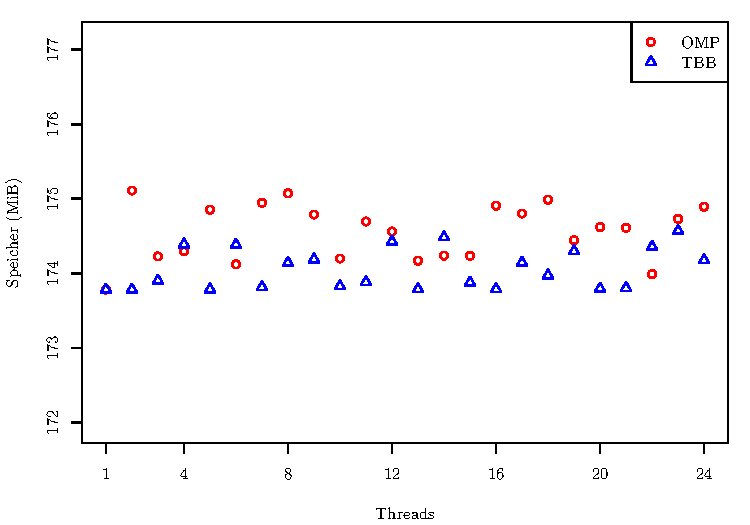
\includegraphics{../messdaten/s14_memory.pdf}
\caption{Speicherverbrauch (Stack und Heap) $M_p(n)$, bei $n=843.074$ und $p \in [1;24]$.}
\label{s14_memory}
\end{figure}

\subsection{Messdaten}

Für die Untersuchung des Laufzeitverhaltens wurde jeweils die tatsächliche Laufzeit (\emph{Wall Time}) und die aufgewandte CPU-Zeit gemessen. Die Anzahl der zur Verfügung stehenden Threads wurde von 1 auf 24 erhöht. Um Messfehler und Ausreißer zu vermeiden, wurde jeweils das arithmetische Mittel aus 10 Einzelmessungen gebildet.

Die gemessenen Rohdaten und die R-Skripte zur Auswertung liegen dieser Arbeit auf Datenträger bei.

%\begin{thebibliography}{3}
%	\bibitem{omp08} S. Hoffmann, R. Lienhart: OpenMP - Eine Einf{\"u}hrung in die parallele Programmierung in C/C++
	
%	\bibitem{openmptut} Blaise Barney, Lawrence Livermore National Laboratory: OpenMP Tutorial \\ https://computing.llnl.gov/tutorials/openMP/ \\ \textit{abgerufen am 24.11.2012}
%\end{thebibliography}

\end{document}
